Det å søke på enten internships eller fast jobb er absolutt ikke lett, men jeg liker å tenke at kvantitet er viktigere enn kvalitet. Det er fordi det kan være svært mange tilfeldigheter som gjør at man selv blir plukket ut blant søkerbunken og da handler det heller om å være i så mange søkerbunker som mulig. Samtidig må jo søknaden og CV-en være av en viss kvalitet, slik at man i det hele tatt blir plukket ut. Jeg skal nå snakke litt om hvordan du kan øke oddsen din mtp. CV og søknad. 

\begin{remark}
    \textbf{PERSPEKTIVER} Det er viktig å søke med riktig forventning. For deg som søker så syntes du hele prosessen er super duper viktig. Du har brukt en uke på CV-en og enda en uke på søknad. Du har kanskje fått foreldre, tanter og onkler til å lese gjennom, og etter en måned får du avslag. Det er også en automatisk mail som går til resten av klassen din som også kanskje har søkt på det samme. Se for deg hvordan den som rekrutterer har det. De har kanskje drevet med dette i 5 år, og hvert år kommer det over 500 søknader på de samme 10 stillingene. Hvor mange sekunder tror du de setter av til hver søknad? Kanskje de må være veldig strenge i år da de økonomiske rammene gjør at de kun kan ta imot 5 interns, når de ifjor tok imot 20. Kanskje de bare skal ha én fra MTKJ, og blant søkerne så møtte de han ene på stand og føler han er relativt safe å invitere på intervju. Kanskje de er venner med foreldrene til noen andre. Eller kanskje de har stått opp på feil side av senga og bare vil få dette unnagjort og plukker derfor bare de første X antall kandidatene til intervju. De rekker kanskje kun å gå gjennom halvparten av bunken før de må dra fra jobb for å hente barna i barnehagen. Neste dag så ser de på lista med kandidater til intervju og tenker <<Det et nok, finner ikke noe særlig bedre>> og forkaster de resterende 250 søknadene. Jeg vil bare få frem her at det kan være så sykt mange faktorer utenom CV og søknaden din som gjør at du ikke blir valgt. Da jeg gikk i 3.klasse sendte jeg ut over 30 søknader og gikk gjennom mange intervjuer før jeg endelig fikk napp. Jeg mener ikke dette for å demotivere, men heller for at du ikke skal få urealistiske forventninger. 
\end{remark}




\section{CV-tips og CV-mal}

Det finnes utrolig mange CV-maler der ute og sikkert mange andre som er bedre enn min (som jeg har kokt og endra på). Likevel vil jeg nevne noen få tips som jeg syntes er essensielle her. Under har jeg også lenket til en del ressurser hos Tekna som anbefales sterkt. 

\begin{figure}[H]
    \centering
    
\includegraphics[width=0.75\linewidth]{images/Tekna-jobb.png}
    \caption{Tekna sine "Digitale karrieretjenester" \url{https://www.tekna.no/student/jobbsoking-for-studenter/}}
    \label{fig:Tekna-jobb}
\end{figure}

\begin{enumerate}
    \item Få med nøkkelord når du skriver beskrivelser. CV-er blir ofte sendt gjennom et program (ATS-program) som scanner etter visse nøkkelord og påvirker sannsynligheten for å bli valgt ut. 
    \item Ikke ta som selvfølge at vedkommende fra HR vet hva studiet ditt går ut på. Derfor må du gjøre dem klar over hva DU kan bidra med. 
    \item Skryt om deg selv! Har du vært kasserer i HC så har du hatt ansvar for flere millioner kroner. Har du vært studass, så har du sikkert rettet over 300 øvinger. Har du vært en eller annen leder for en komité, så har du hatt ledelsesansvar for et team med eksempelvis 10 personer. Hvis du har oppnådd noe konkret, så skriv det på CV-en din også. 
    \item Hold det kort, ikke skriv hele livshistorien din, men heller lag en punktliste over det mest essensielle. Du trenger ikke å utdype <<Servitør>>, men heller at du har hatt personalansvar eller oppnådd noe i stillingen. Om du ikke har oppnådd noe konkret, kan du bruke <<erfaring med kundeservice>> eller andre nøkkelord i stedet. 
\end{enumerate}

Hvis du ikke vil høre på meg, så har NIRAS 5 gode tips til en CV som vist på bildet under:

\begin{figure}[H]
    \centering
    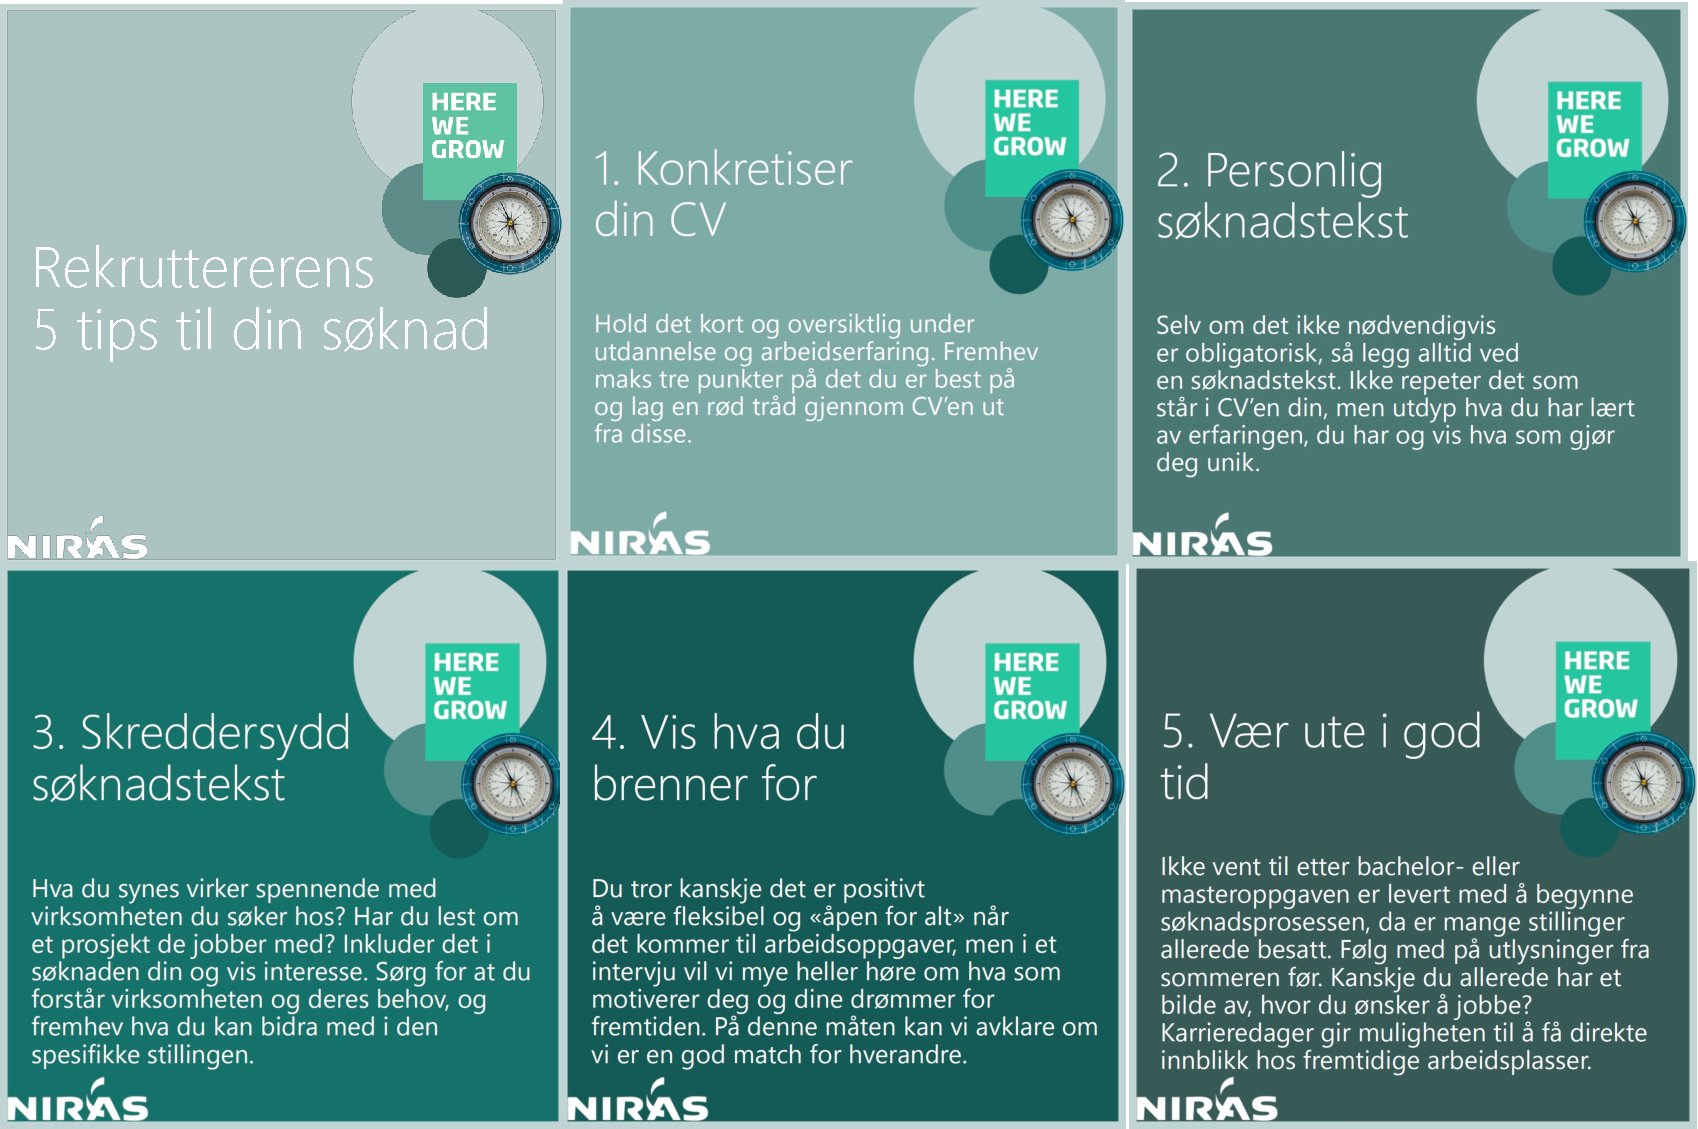
\includegraphics[width=0.8\linewidth]{images/CV-tips.pdf}
    \caption{NIRAS sine CV-tips}
\end{figure}


\begin{figure}[H]
    \centering
    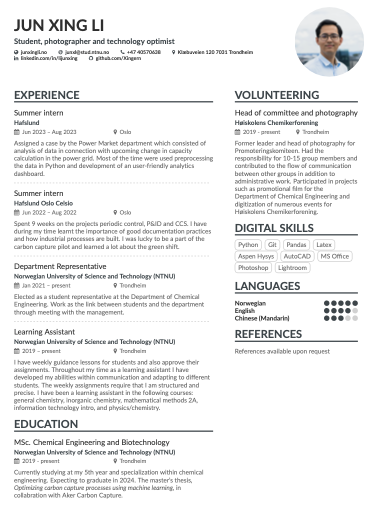
\includegraphics[width=0.5\linewidth]{images/CV-example.png}
    \caption{Eksempel på CV-mal jeg bruker. Malen ligger på Github: \url{https://github.com/Xingern/karriereguide}}
    \label{fig:enter-label}
\end{figure}



\section{Søknadsbrev}

Jeg mener jo at det å søke på internships og jobber ofte handler om kvantitet over kvalitet. Derfor kan det være lurt å strukturere søknaden slik at man kan gjenbruke mye, men likevel ha en spesifikk del for stillingen man søker på. Jeg bruker Overleaf for å lage CV-en min og Tekna sin <<CV-bygger>> for å lage en fin søknadstekst. Jeg liker å strukturere ting etter avsnitt:

\begin{enumerate}
    \item Begynn med en kort grunn for hvorfor du søker denne stillingen. (Her kan du si at du har gledet deg til å søke på stillingen siden du var på bedpres i fjor)
    \item Introduksjon av deg selv og studiebakgrunn. Hvorfor er bakgrunnen din relevant for stillingen? Hva konkret fra studiet er relevant? Laberfaring? Dataanalyse? Problemløsing?
    \item Snakk om hva du har lært fra tidligere internships og andre jobber, gjerne konkrete faglige ting. Her er det faglig relevans utenom studiet som gjelder.
    \item Hvorfor akkurat dette selskapet? Les deg opp om dem, nevn evt. samtale på stands, lest om dem i nyheter osv. Gjør det så personlig som mulig. Har du utenlandske foreldre og selskapet har kontor der også? Hva syntes du er spesielt kult med denne bedriften?
    \item Dette avsnittet skal snakke om hva som er relevant utenom studiet, og da nevner jeg spesielt verv. Verv bidrar ofte ikke faglig, men veldig på det dagligdagse. Highlight derfor de <<årene>> du har hatt med verv, teamarbeid, mailskriving og hvordan du balanserte mellom studier og verv. 
    \item Siste pitch på hvorfor selskapet er der du vil havne og en kort oppsummering av deg og det som har blitt nevnt tidligere. 
\end{enumerate}

\begin{figure}[H]
    \centering
    \includegraphics[width=0.6\linewidth]{images/Søknadsbrev_eksempel.png}
    \caption{Eksempel på søknadsstruktur jeg bruker. Flere eksempler ligger på Github: \url{https://github.com/Xingern/karriereguide/tree/main/cover_letters}}
\end{figure}

For å presentere typiske søknader så har jeg lagt ved 4 søknadsbrev som har endt i et positivt utfall. De er skrevet av meg selv, og er derfor basert på mine personlige erfaringer og opplevelser, så ikke fosskok, men heller hent inspirasjon fra disse. Og for guds skyld, ikke bruk ChatGPT til å skrive søknader. Det ChatGPT derimot er flink til, er å omformulere og gjerne gi overordnede forslag. I den anledning vil jeg også komme med et flott forslag jeg selv har fått: Hvis du skal skrive en søknad på maks 250 ord, så er følgende struktur ganske flott:

\begin{enumerate}
    \item Start med en kort introduksjon, noe som ligner på hva som er nevnt over. Derimot skal siste setning nevne at de tre neste punktene er 3 grunner for hvorfor bedriften skal velge deg.
    \item Grunn nr.1 kan handle om hvorfor du er egnet mtp. det faglige.
    \item Grunn nr.2 kan handle om hvorfor denne bedriften er spesiell for deg.
    \item Grunn nr.3 kan handle om personlig motivasjon.
    \item Kort oppsummering av de forrige 3 punktene.
\end{enumerate}

Eksempel på en slik <<pitchsøknad>> ligger også på GitHub. 






\section{Evnetest}

Mange søkeres verste mareritt. Jeg anbefaler å se på evnetester som ulike eksamenssett. Det er alltid de samme spørsmålene som går igjen, og du kan øve deg på det meste. De aller fleste bruker AON Maptq og disse finnes det mange tips om rundt omkring på nettet.

\begin{figure}[H]
    \centering
    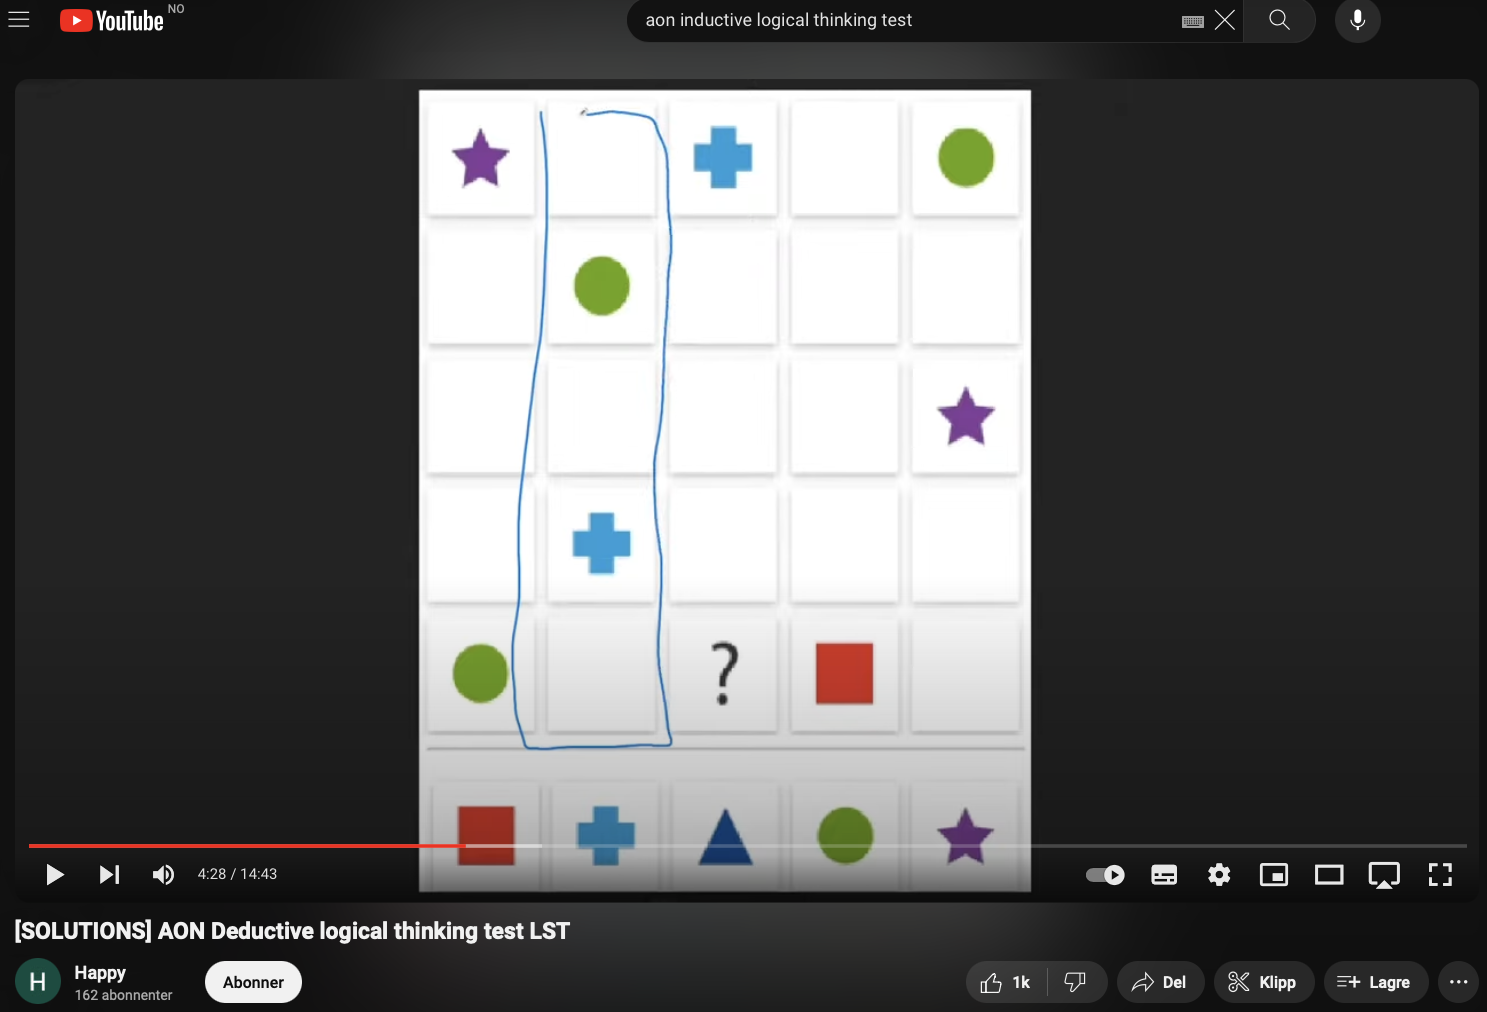
\includegraphics[width=0.8\linewidth]{images/aon.png}
    \caption{Du finner YouTube-videoer på samtlige evnetester der ute så du kan alltid få en sneak peak.}
\end{figure}

Her kan jeg nevne et eksempel fra noen bekjente. Vedkommende hadde søkt en stilling og fikk utdelt en evnetest. En av oppgavene innehold en rekke faner med grafer, tabeller og ulik tekst. Spørsmålene var rettet mot all informasjonen som ble presentert, noe som virker overveldende. Uka etter fikk vedkommende en evnetest fra en annen stilling, hvor en av oppgavene var det samme som forrige uke! Alt av tabeller og grafer var jo allerede kjent og vedkommende klarte seg utmerket på evnetesten. 



\section{Intervju}

Det finnes igjen utallige mange måter et intervju kan foregå på. Jeg vil bare nevne at det er mengdetrening som er nøkkelen og det hjelper utrolig mye å ha søkt på internships i 3.klasse uten hell, fordi da er du veldig godt forberedt til 4.klasse. 

\begin{enumerate}
    \item Det er viktig å vite hvem du skal på intervju med. Det gjelder både bedriften, men også de du møter på intervjuet. Det er eksempelvis stor forskjell på å delta på intervju med HR versus avdelingsleder med ingeniørbakgrunn. Derfor er rådet her at du burde søke opp navnene på intervjuinnkallingen på LinkedIn. Har vedkommende tidligere gått MTKJ så trenger du antageligvis ikke bruke så mye tid på å forklare studiet.
    \item Øv på de typiske spørsmålene. Spørsmål som <<hvem er du>> og <<hvorfor du søker hos oss>> og lignende dukker ofte opp. Det finnes mange lister med typiske spørsmål ute på nettet, så bruk litt tid på å øve på noen av dem.
\end{enumerate}




\section{Caseintervju}

Mange bedrifter opererer med caseintervju som et 2.gangsintervju. Dette er spesielt vanlig blant de store konsulenthusene da caseløsning er en sentral del av arbeidshverdagen. 

\begin{enumerate}
    \item Hos mange IT-konsulenthus så kjøres det kodeintervjuer. Det kan bety at man enten skal kode noe i forkant av intervjuet eller mens det pågår. Det viktigste er å vise frem tankegangen din og det er fullstendig lov å feile. Det kreves heller ikke all verdens kodeerfaring og forkunnskaper fra ITGK er som oftest tilstrekkelig. 
    \item Hvis du får tilbud om intervju med noen av de management-konsulenthusene så er caseintervju svært vanlig. Det innebærer et kundecase på gjerne 30 min forberedelse og 30 min presentasjon av resultatene man har kommet frem til. Det finnes mange eksempler på slike caser på nettet, men det viktigste tipset er å begrunne hvorfor man gjør som man gjør. Det finnes ingen riktige svar og så lenge du begrunner godt så kan man konkludere med hva som helst. 
\end{enumerate}